\documentclass[../../main/thesis_msc.tex]{subfiles}


\begin{document}

	\chapter{Results}
	
		
		
			\section{Single helium stars}
			
				\subsection{Internal structure - Core growth}
				
					\subsubsection{Evolution in the mass range $2.0$ M$_{\odot}$ to $2.8$ M$_{\odot}$}
					
					\subsubsection{Evolution in the mass range $2.9$ M$_{\odot}$ and above}
				
				
				\subsection{Radius evolution}
					During its lifetime, the radius of a star will vary depending on its evolutionary stage. The reason behind these changes is the occurance of several instabilities ranging from the natural exhaustion of a burning nuclear fuel to the violent, non-runaway ignition of matter in a shell (shell flash). 
					
					Following the depletion of hydrogen in the center and the subsequent removal of the hydrogen mantle, the exposed helium core will contract as a whole trying to reach higher temperatures for helium to ignite as can be seen in \hyperref[fig:radii_singles]{Fig 3.1}. Naturally, the less massive a star is, the more it needs to contract before the right conditions for helium ignition are reached.
				
					\begin{figure}[h]
						\centering
						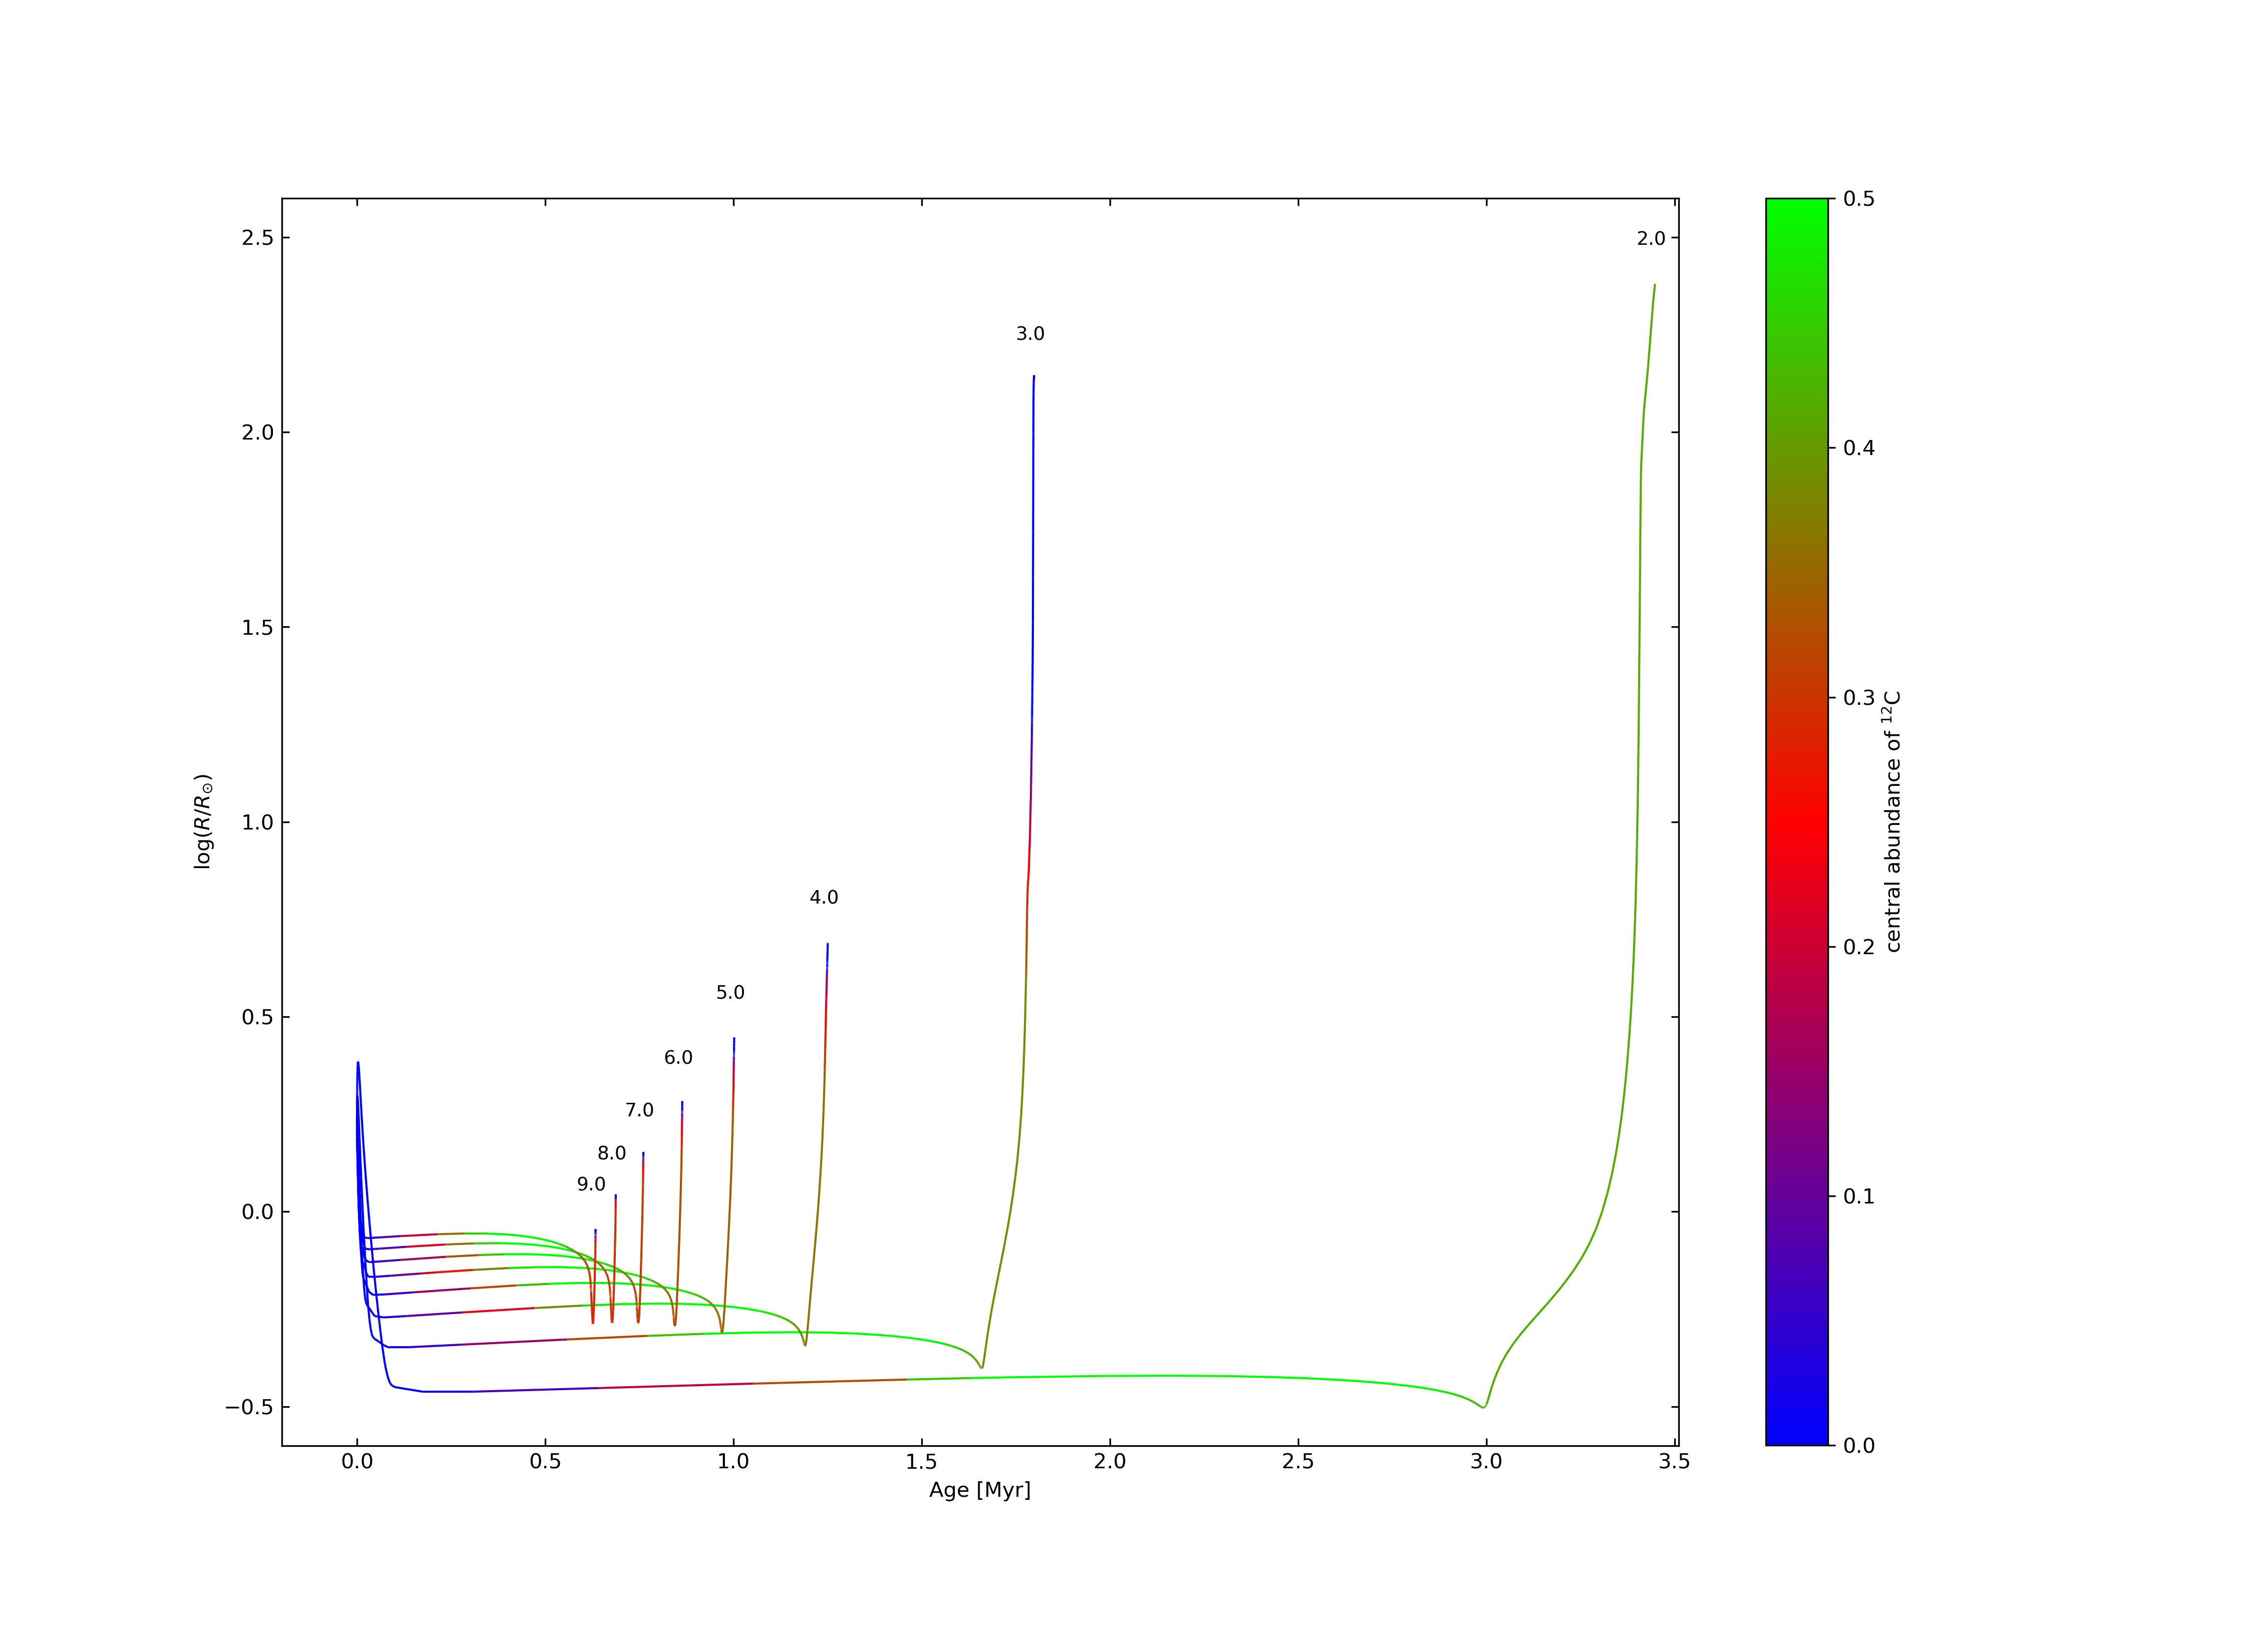
\includegraphics[scale=0.4]{../figures/chapter3/radius_evolution_gradient.png}
						\caption{Evolution of stellar radii as a function of time until central carbon depletion. The colour map indicates the evolutionary stage of every helium star in terms of central abundance of carbon whilst the numbers on top of each curve denote the initial mass of the star.}
						\label{fig:radii_singles}
					\end{figure}
					
					When core helium burning comes to an end, the main source of energy comes from a He-burning shell surrounding the inert core which resumes its contraction phase until the on-centre carbon ignition; this happens for all stellar models depicted in \hyperref[fig:radii_singles]{Fig 1.3}, with the exception of the lowest mass model (M$_{i} = 2.0$ M$_{\odot}$) for which carbon is ignited off-centre. During the He-shell burning phase, and the subsequent core carbon burning phase, the radius of the stars increases until the carbon in the centre is consumed.
					
					As expected, the more massive stars exhaust their nuclear fuel supply and reach advanced burning stages more rapidly than lower mass stars; this is clearly illustrated in \hyperref[fig:radii_singles]{Fig 1.3}. However, by taking a closer look at this figure, we observe a more important behaviour that is related to the mass of the helium stars: the degree at which the radius expands has a tendency to increase as the initial mass of the star decreases. This has important consequences when it comes to helium stars that are part of a binary system, since it indicates that lower mass stars can fill their Roche-lobe and initiate mass transfer at larger orbital separations compared to the more massive ones. Additionally, the inflated envelope is more loosely bound to the core making these stars prone to sub-surface thermal instabilities such as thin-shell burning, or opacity-driven instabilities that could potentially remove a significan amount of surface material. % Last sentence needs reconsideration
				
				
				\subsection{Abundance profiles}	
			
			
			
			\section{Neutron star + helium star binaries}




\end{document}